\section{Empirical evaluation: further details}\label{appendix:empirical-evaluation-details}

In this section with give further details about the synthetic and real-data experiments presented in Section \ref{sec:experiments}.

\subsection{Synthetic experiments}



\subsubsection{Analytical expressions for divergences between two Gaussians}\label{appendix:toy-exps}

The closed form expression for the $\chi^2$-divergence between two $d$-variate normal distributions can be found in Lemma 1 of~\cite{NielsenN14}:
\begin{lemma}\label{lemma:chi-squared-closed-form}
\begin{align*}
&\chi^2\bigl( \mathcal{N}(\mu_1, \Sigma_1), 
\mathcal{N}(\mu_2, \Sigma_2)\bigr)
=
\frac{\mathrm{det}(\Sigma_1^{-1})}{\sqrt{\mathrm{det}(2\Sigma_1^{-1} - \Sigma_2^{-1})\mathrm{det}(\Sigma_2^{-1})}}
\exp\left(
\frac12\mu_2'\Sigma_2^{-1}\mu_2 
-\mu_1'\Sigma_1^{-1}\mu_1 
\right)
\times\\
&\times\exp\left(
-\frac14(2\mu_1' \Sigma_1^{-1} - \mu_2' \Sigma_2^{-1})
\bigl(\frac12 \Sigma_2^{-1} - \Sigma_1^{-1}\bigr)^{-1}
(2\Sigma_1^{-1}\mu_1 - \Sigma_2^{-1}\mu_2)
\right) - 1.
\end{align*}
\end{lemma}
As a corollary, the following also holds:
\begin{corollary}
Chi square divergence between two $d$-variate Gaussian distributions both having covariance matrices proportional to identity can be computed as:
\[
\chi^2\bigl( \mathcal{N}(\mu, \sigma^2 I_d), \mathcal{N}(0, \beta^2 I_d)\bigr)
=
\left(\frac{\beta^2}{\sigma^2\sqrt{2\beta^2/\sigma^2 - 1}}\right)^d
e^{\frac{\|\mu\|^2}{2\beta^2 - \sigma^2}}
- 1
\]
assuming $2\beta^{2} > \sigma^{2}$. 
Otherwise the divergence is infinite.
\end{corollary}

The squared Hellinger divergence between two Gaussians is given in \cite{pardo2005statistical}:

\begin{lemma}
\begin{align*}
&H^2\bigl( \mathcal{N}(\mu_1, \Sigma_1), 
\mathcal{N}(\mu_2, \Sigma_2)\bigr) \\
&\qquad = 1 - \frac{ \det (\Sigma_1)^{1/4} \det (\Sigma_2) ^{1/4}} { \det \left( \frac{\Sigma_1 + \Sigma_2}{2}\right)^{1/2} }
              \exp\left\{-\frac{1}{8}(\mu_1 - \mu_2)^T 
              \left(\frac{\Sigma_1 + \Sigma_2}{2}\right)^{-1}
              (\mu_1 - \mu_2)              
              \right\}.
\end{align*}
\end{lemma}

The $\KL$-divergence between two $d$-variate Gaussians is:
 
\begin{lemma}
\begin{align*}
\KL\bigl( \mathcal{N}(\mu_1, \Sigma_1), 
\mathcal{N}(\mu_2, \Sigma_2)\bigr) = \frac{1}{2} \left( \text{tr}\left(\Sigma_2^{-1} \Sigma_1\right)
+ (\mu_2  - \mu_1)^\intercal \Sigma_2^{-1}(\mu_2 - \mu_1) - d + \log\frac{|\Sigma_2|}{|\Sigma_1|}
\right).
\end{align*}
\end{lemma}



\subsubsection{Further experimental details}

We take $Q^\lambda_{Z|X=x} = \mathcal{N}\left(A_\lambda x + b_\lambda, \epsilon^2 I_d \right)$ and $P_X = \mathcal{N}\left(0, I_{20} \right)$.
This results in $Q^\lambda_Z = \mathcal{N}\left(b_\lambda,  A_\lambda A_\lambda^\intercal + \epsilon^2 I_d \right)$. We chose $\epsilon=0.5$ and used $\lambda \in [-2,2]$. $P_Z = \mathcal{N}(0, I_d)$.

$A_\lambda$ and $b_\lambda$ were determined as follows:
Define $A_1$ to be the $(d, 20)$-dimensional matrix with 1's on the main diagonal, and let $A_0$ be similarly sized matrix with entries randomly sampled i.i.d.\: unit Gaussians which is then normalised to have unit Frobenius norm. 
Let $v$ be a vector randomly sampled from the $d$-dimensional unit sphere.
We then set
$A_\lambda=\frac{1}{2} A_1 + \lambda A_0$ and $b_\lambda= \lambda v$.

$A_0$ and $v$ are sampled once for each dimension $d{\in}\{1,4,16\}$, such that the within each column of Figure~\ref{fig:synthetic-exps}, the distributions used are the same.







\subsection{Real-data experiments}\label{appendix:real-data-experiments-additional}

\subsubsection{Variational Autoencoders (VAEs) and Wasserstein Autoencoders (WAEs)}\label{appendix:intro-vae-wae}

Autoencoders are a general class of models typically used to learn compressed representations of high-dimensional data.
Given a \emph{data-space} $\mathcal{X}$ and low-dimensional \emph{latent space} $\mathcal{Z}$, the goal is to learn an \emph{encoder} mapping $\mathcal{X}\to\mathcal{Z}$ and \emph{generator} (or \emph{decoder}\footnote{In the VAE literature, the encoder and generator are sometimes referred to as the \emph{inference network} and \emph{likelihood model} respectively.}) mapping $\mathcal{Z}\to\mathcal{X}$.
The objectives used to train these two components always involve some kind of reconstruction loss measuring how corrupted a datum becomes after mapping through both the encoder and generator, and often some kind of regularization.

Representing by $\theta$ and $\eta$ the parameters of the encoder and generator respectively, the objective functions of VAEs and WAEs are:

\begin{align*}
    L^{\text{VAE}}(\theta, \eta) &= \E_X \left[ \E_{q_\theta(Z|X)} \log p_\eta(X|Z) + \KL\left( Q^\theta_{Z|X} \| P_Z) \right) \right]\\
    L^{\text{WAE}}(\theta, \eta) &= \E_X \E_{q_\theta(Z|X)} c(X, G_\eta(Z)) + \lambda \cdot D(Q^\theta_Z \| P_Z)
\end{align*}

For VAEs, both encoder $Q^\theta_{Z|X}$ and generator $p_\eta$ are \emph{stochastic} mappings taking an input and mapping it to a distribution over the output space.
In WAEs, only the encoder $Q^\theta_{Z|X}$ is stochastic, while the generator $G_\eta$ is deterministic.
$c$ is a cost function, $\lambda$ is a hyperparameter and $D$ is any divergence.

A common assumption made for VAEs is that the generator outputs a Gaussian distribution with fixed diagonal covariance and mean $\mu(z)$ that is a function of the input $z$.
In this case, the $\log p_\eta(X|z)$ term can be written as the $l^2_2$ (i.e. square of the $l_2$ distance) between $X$ and its reconstruction after encoding and re-generating $\mu(z)$.
If the cost function of the WAE is chosen to be $l^2_2$, then the left hand terms of the VAE and WAE losses are the same. 
That is, in this particular case, $L^{\text{VAE}}$ and $L^{\text{WAE}}$ differ only in their regularizers.

The penalty of the VAE was shown by \cite{hoffman2016elbo} to be equivalent to $\smash{\KL(Q^\theta_Z \| P_Z) + I(X,Z)}$ where $I(X,Z)$ is the mutual information of a sample and its encoding.
For the WAE penalty, there is a choice of which $\smash{D(Q^\theta_Z \| P_Z)}$ to use; it must only be possible to practically estimate it.
In the experiments used in this paper, we considered models trained with the Maximum Mean Discrepency (MMD) \cite{gretton2012kernel}, a kernel-based distance on distributions, and a divergence estimated using a GAN-style classifier \cite{goodfellow2014generative} leading to WAE-MMD and WAE-GAN respectively, following \cite{tolstikhin2017wasserstein}.

\subsubsection{Further experimental details}

We took a corpus of VAE, WAE-GAN and WAE-MMD models that had been trained with a large variety of hyperparameters including learning rate, latent dimension (32, 64, 128), architecture (ResNet/DCGAN), scalar factor for regulariser, and additional algorithm-specific hyperparameters: kernel bandwidth for WAE-MMD and learning rate of discriminator for WAE-GAN.
In total, 60 models were trained of each type (WAE-MMD, WAE-GAN and VAE) leading to 180 models in total.

The small subset of six models exposed in Figures~\ref{fig:real-exps} and \ref{fig:real-exps-hsq} were selected by a heuristic that we next describe. However, we note that qualitatively similar behaviour was found in all other models tested, and so the choice of models to display was somewhat arbitrary; we describe it nonetheless for completeness.

Recall that the objective functions of WAEs and VAEs both include a divergence between $Q^\theta_Z$ and $P_Z$.
We were interested in considering models from the two extremes of the distribution matching: some models in which $Q^\theta_Z$ and $P_Z$ were close, some in which they were distant.

To determine whether $Q^\theta_Z$ and $P_Z$ in a model are close, we made use of FID \cite{heusel2017gans} scores as a proxy that is independent of the particular divergences for training.
The FID score between two distributions over images is obtained by pushing both distributions through to an intermediate feature layer of the \emph{Inception} network.
The resulting push-through distributions are approximated with Gaussians and the \emph{Fr\'echet} distance between them is calculated.
Denote by $G_\#(Q^\theta_Z)$ the distribution over reconstructed images, $G_\#(P_Z)$ the distribution over model samples and $Q_X$ the data distribution, where $G$ is the generator and $\#$ denotes the push-through operator. 
The quantity $\text{FID}\left(Q_X, G_\#(Q^\theta_Z)\right)$ is a measure of quality (lower is better) of the reconstructed data,
while $\text{FID}\left(Q_X, G_\#(P_Z)\right)$ is a measure of quality of model samples.

The two FID scores being very different is an indication that $P_Z$ and $Q^\theta_Z$ are different.
In contrast, if the two FID scores are similar, we cannot conclude that $P_Z$ and $Q^\theta_Z$ are the same, though it provides some evidence towards that fact.
Therefore, in order to select a model in which matching between $P_Z$ and $Q^\theta_Z$ is poor, we pick one for which $\text{FID}\left(Q_X, G_\#(Q^\theta_Z)\right)$ is small but $\text{FID}\left(Q_X, G_\#(P_Z)\right)$ is large (good reconstructions; poor samples).
In order to select a model in which matching between $P_Z$ and $Q^\theta_Z$ is good, we pick one for both FIDs are small (good reconstructions; good samples). 
We will refer to these settings as \emph{poor matching} and \emph{good matching} respectively.

Our goal was to pick models according to the following criteria. 
The six chosen should include: two from each model class (VAE, WAE-GAN, WAE-MMD), of which one from each should exhibit poor matching and one good matching; two from each dimension $d\in\{32, 64, 128\}$; three with the ResNet architecture and three with the DCGAN architecture.
A set of models satisfying these criteria were selected by hand, but as noted previously we saw qualitatively similar results with the other models.

\subsubsection{Additional results for squared Hellinger distance}\label{appendix:sq-hellinger-results}

Figure~\ref{fig:real-exps-hsq} we display similar results to those displayed in Figure~\ref{fig:real-exps} of the main paper but with the $H^2$-divergence instead of the KL.
An important point is that $H^2(A,B) \in [0, 2]$ for any probability distributions $A$ and $B$,
and due to considerations of scale we plot the estimated values $\log\big(2 - \hat{D}^M_{H^2}(\hat{Q}^N_Z \| P_Z)\big)$.
Decreasing bias in $N$ of RAM-MC therefore manifests itself as the lines \emph{increasing} in Figure~\ref{fig:real-exps-hsq}. 
Concavity of $\log$ means that the reduction in variance when increasing $M$ results in RAM-MC with $M{=}1000$ being above RAM-MC with $M{=}10$.
Similar to those presented in the main part of the paper, these results therefore also support the theoretical findings of our work.

We additionally attempted the same experiment using the $\chi^2$-divergence but encountered numerical issues.
This can be understood as a consequence of the inequality $e^{\KL(A, B)} - 1 \leq \chi^2(A,B)$ for any distributions $A$ and $B$. 
From Figure~\ref{fig:real-exps} we see that the $\KL$-divergence reaches values higher than $1000$ which makes the corresponding value of the $\chi^2$-divergence larger than can be represented using double-precision floats.

\begin{figure}
\begin{center}
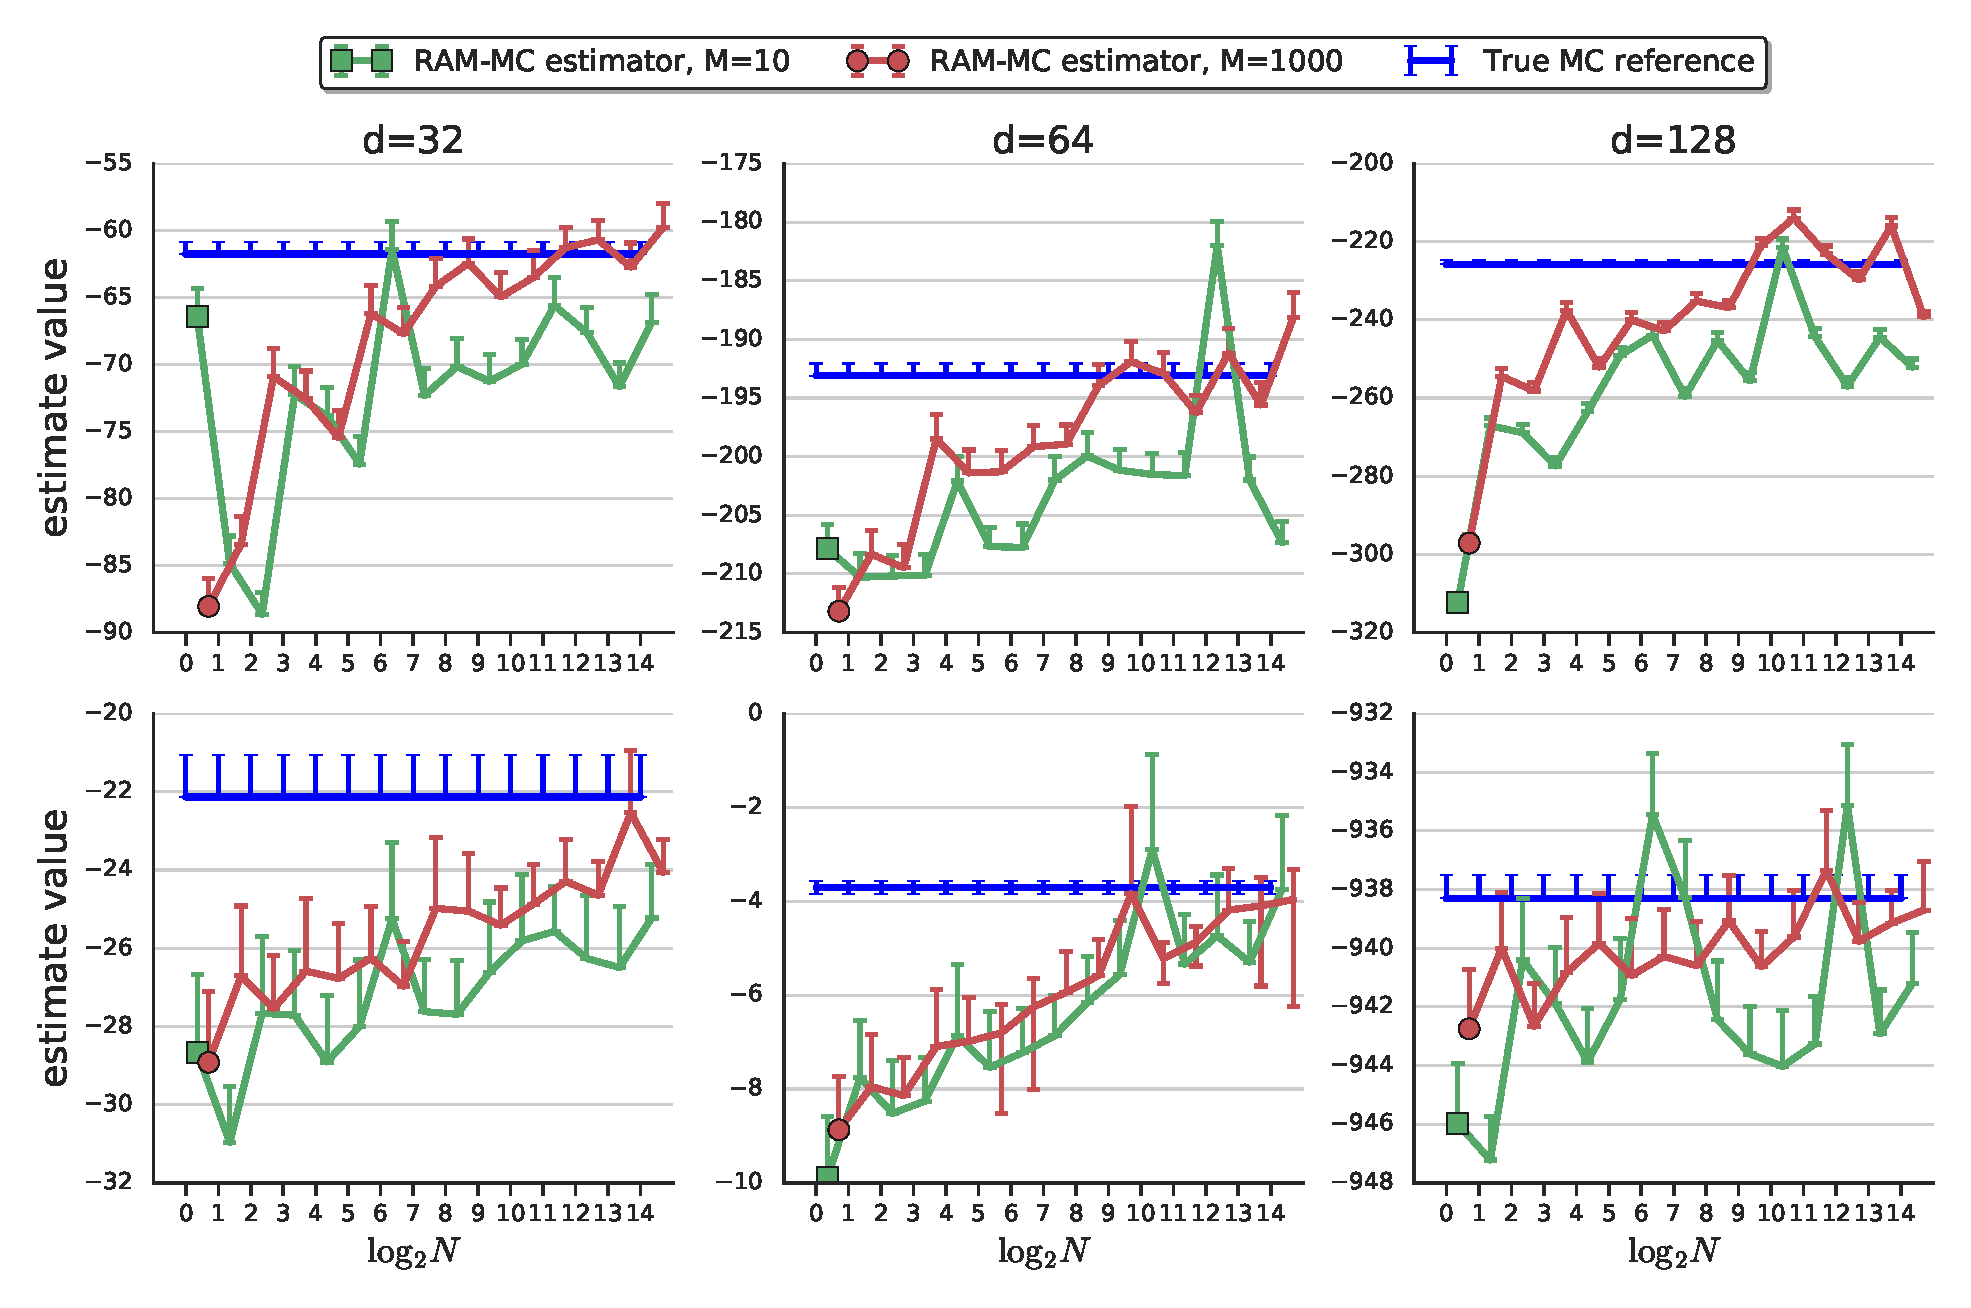
\includegraphics[width=1.\textwidth, height=0.615\textwidth]{pics/NeurIPS_wae_exps_plot_hsq.pdf}
\end{center}
\caption{\label{fig:real-exps-hsq}
Estimating $H^2(Q_Z^\theta \| P_Z)$ in pretrained autoencoder models with RAM-MC as a function of $N$ for $M=10$ ({\bf \textcolor{green!65!blue}{green}}) and $M{=}1000$ ({\bf \textcolor{red}{red}}) compared to ground truth ({\bf\textcolor{blue}{blue}}).
Lines and error bars represent means and standard deviations over 50 trials.
Plots depict $\log\big(2 - \hat{D}^M_{H^2}(\hat{Q}^N_Z \| P_Z)\big)$ since $H^2$ is close to 2 in all models.
Omitted lower error bars correspond to error bars going to $-\infty$ introduced by $\log$.
Note that the approximately \emph{increasing} behaviour evident here corresponds to the expectation of RAM-MC \emph{decreasing} as a function of $N$. 
Due to concavity of $\log$, the decrease in variance when increasing $M$ manifests itself as the {\bf \textcolor{red}{red}} line ($M{=}1000$) being consistently above the {\bf \textcolor{green!65!blue}{green}} line ($M{=}10$).
}
\end{figure}